%==============================================================================
% 13th IFAC Symposium on Fault Detection, Supervision and Safety for Technical
% Processes (SAFEPROCESS 2027), Delft, 29 June - 2 July 2027.
% Paper deadline: 31 October 2026.  Submission via https://ifac.papercept.net
%
% IFAC uses SINGLE-BLIND review: author names and affiliations stay on the paper.
% Do not anonymise.
%
% BUILD
%   pdflatex safeprocess2027_final && pdflatex safeprocess2027_final
%   Fig. 1 (figures/fig_tiebreak.pdf) and Fig. 2
%   (figures/fig_signatures_column.pdf) are built by make_figures.py at the
%   repository root.
%
% CLASS FILE
%   ifacconf.cls ships from IFAC, not from CTAN/TeX Live:
%     https://www.ifac-control.org/conferences/author-guide
%   It is not in this repository.  tools/ifacconf_local.cls is a LOCAL
%   APPROXIMATION written only so the draft can be compiled and page-counted.
%   To build, copy it next to this file as ifacconf.cls, or drop in the
%   official class (this source needs no other change).  Verify the page count
%   again with the official class -- the official geometry will differ.
%
% LENGTH
%   6 pages final, up to 8 for review.  Cut list if over, in this order:
%   the Sec. 4 route paragraph's tau sentence, Table 2's permuted column, the
%   Sec. 8.2 foam-collision sentence.
%
% PROVENANCE
%   Every number here traces to results/*.json, except in Sec. 3: the dataset
%   counts (2122 / 755 / 1367 / 948 / 419 cycles) are voraus-AD's own, and the
%   detector's AUROC is computed by mvtflow/train.py from the raw parquet and
%   written to results/detector_metrics.json (not shipped).  Main sources:
%   baselines.json (Table 1, Sec. 5: prior_vs_retrieval, tie_robust,
%   tiebreak_exact, balanced_recall_expected, set_valued, constant_router),
%   distinguishability_results.json (Sec. 4), repair_results.json (Table 2,
%   Sec. 6), certificate_checks.json (Secs. 6 and 8), protocol_check.json
%   (Sec. 7), held_out_seeds.json (Sec. 3).
%==============================================================================
\documentclass{ifacconf}

% T1 fixes the accented surnames in the bibliography: under OT1 the accent and
% the base letter are separate glyphs in the PDF text layer, which breaks
% full-text search and author indexing on IFAC-PapersOnLine.
% lmodern is NOT optional alongside it.  With T1 and no Type 1 EC fonts on the
% system, LaTeX silently falls back to METAFONT bitmaps, the PDF carries Type 3
% fonts, and PaperCept refuses the upload ("Bitmapped Font error").  It also
% restores the fi/fl/ff ligatures in the PDF text layer.
% VERIFY WITH: pdffonts safeprocess2027_final.pdf -- there must be no "Type 3" row.
\usepackage[T1]{fontenc}
\usepackage{lmodern}
\usepackage{graphicx}
\usepackage{booktabs}
\usepackage[hidelinks]{hyperref}
% the repository URL is long and lives in a narrow column; let it break anywhere
\usepackage{xurl}
\graphicspath{{figures/}}

\begin{document}

\begin{frontmatter}

\title{Structural Non-Isolability in Knowledge-Based Robot Fault Diagnosis:
Tie-Break Intervals and Grouped Validation}

% IFAC is single-blind: author names and affiliations stay on the paper.
% CHECK: confirm how the second author prefers to be listed (Christy Jie Liang
% vs Jie Liang) and whether a School-level line should replace the Faculty one.
% TODO: if the work is funded, IFAC puts the acknowledgement in \thanks{} on the
% title, e.g. \title{...}\thanks{This work was supported by ...}
\author[uts]{Chenxuan Zhou}
\author[uts]{Christy Jie Liang}
\address[uts]{Faculty of Engineering and Information Technology,
University of Technology Sydney, Ultimo, NSW 2007, Australia
(e-mail: chenxuan.zhou@student.uts.edu.au, jie.liang@uts.edu.au).}

\begin{abstract}
On the public voraus-AD robot benchmark we evaluate a diagnosis layer that
scores the 14 failure modes of a hand-written FMEA knowledge base against
per-signal deviations from normal operation. In 514
of 755 anomalous cycles two or three modes share the top score, always inside
one of four groups whose declared signatures are identical or contain one
another. Over the 12 tie-break orders that matter, top-1 accuracy ranges from
0.119 to 0.200; a prevalence prior that reads no evidence scores 0.187 and is
better on top-3, top-5, mean reciprocal rank and group accuracy under every
order. We therefore report the non-isolable group and search statistics of the
existing signals for one that separates it. For the load-torque group the sign
of the deviation separates the members (held-out accuracy 0.840 against 0.562);
the other groups are inconclusive, undetermined or untestable. The search must
be validated on unseen fault instantiations: under a random split over cycles it
adopts a repair for the collision group that leave-one-setting-out validation
adopts on only 4 of 9 folds, below the majority-class rate. A flat classifier
over the same features is more accurate than the whole pipeline once more than
a few labels are available.
\end{abstract}

% Taken from the SAFEPROCESS official keyword list -- do not substitute
% free-text terms, PaperPlaza routes the paper to a Technical Committee on the
% first keyword.
\begin{keyword}
Fault isolation and root cause analysis, Structural analysis methods,
Diagnosability analysis, Knowledge-based diagnosis, Anomaly detection,
Robotics.
\end{keyword}

\end{frontmatter}

%==============================================================================
\section{Introduction}
%==============================================================================

An anomaly detector on robot telemetry can report that a cycle is abnormal, but
not why. A common way to add a cause is a line-specific FMEA knowledge base:
each failure mode declares the joints it affects and the signal families in
which it shows, a retrieval function scores the modes against the per-signal
deviations of the cycle, and the maintenance technician receives a ranked list
of candidate causes.

This paper measures what such a list can decide on the public voraus-AD
benchmark \citep{voraus}. The declarations of the knowledge base form a fault
signature matrix in the sense of \citet{blanke}. In this matrix nine of the
fourteen failure modes share their signature with another mode: six have
identical columns, and in a group of three one column contains the other two.
The scoring function is continuous, but it does not separate these modes. It gives them exactly the same score: in 514 of 755 anomalies two or
three modes share the highest score, and the reported answer is then decided by
the order in which the modes are listed (Fig.~\ref{fig:tiebreak}).

Two consequences do not depend on this knowledge base. The first concerns the
reference for judging accuracy. Our earlier evaluation of this layer compared
top-1 accuracy with uniform chance. When fault frequencies are skewed, the
appropriate reference is a prevalence prior, which ranks the modes by their
frequency in the training data and gives this ranking for every cycle. On
voraus-AD the prior is better than the retrieval on every measure that does not
depend on the tie-break order (Sec.~\ref{sec:baselines}).

The second concerns validation. The \texttt{setting} field of voraus-AD
identifies a physical fault instantiation, for example one added weight or one
placement of a collision object, and each instantiation is repeated over several
cycles. A random split over cycles puts cycles of the same instantiation into
both the training and the test data. We show that this changes which learned
repair is adopted, not only the reported accuracy (Sec.~\ref{sec:protocol}).
Leakage of this kind is known in machine-learning-based science \citep{kapoor}
and in fault-diagnosis benchmarks \citep{hendriks}; here it enters through the
inner validation that selects the repair. We test both points on voraus-AD only.

\begin{figure}[t]
\centering
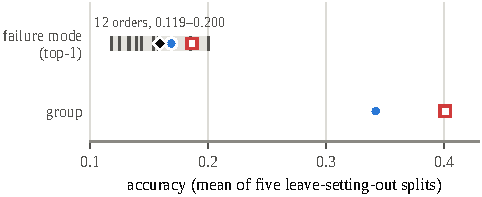
\includegraphics[width=\linewidth]{fig_tiebreak.pdf}
\caption{Top-1 and group accuracy of the retrieval, means over the splits of
Table~\ref{tab:baselines}. Upper row: band and ticks, all 12 relative orders of
the tied modes; circle, declared order; diamond, mean over orders; square,
prevalence prior. Lower row: the group (circle) is the same under every order;
always naming the most frequent group (square) is more accurate.}
\label{fig:tiebreak}
\end{figure}

\emph{Contributions.} (i) The knowledge base analysed as a fault signature
matrix, with non-isolable groups reported instead of broken by a tie-break rule.
(ii) Two references for a ranked candidate list on this benchmark: a prevalence
prior and the exact range of top-1 accuracy over tie-break orders. (iii) A
search over named statistics of the existing signals for one that separates a
group, reported as a certificate with held-out evidence, controls and a cost
class. (iv) Evidence that grouping the validation by fault instantiation changes
which repair is adopted. (v) A flat classifier that outperforms our pipeline,
with the label budget from which it does.

%==============================================================================
\section{Fault signatures and isolability}
%==============================================================================

Structural diagnosability analysis determines, before any data are seen, which
faults a diagnosis system can separate, using the incidence structure of tests
and fault modes \citep{blanke,krysander_mso}. The standard object is the fault
signature matrix, whose rows are tests or residuals and whose columns are fault
modes. Under the exoneration assumption two modes are non-isolable exactly when
their columns coincide. Without it isolability is directional: a mode whose
column is contained in another mode's column cannot be isolated from that mode
\citep{krysander,cordier}. The analysis has been applied to public process
benchmarks \citep{damadics}, extended to graded distinguishability under noise
\citep{jung}, and is still developed \citep{tm_wotawa}.

When the signatures do not separate the faults, both FDI signature matching and
consistency-based diagnosis in the DX tradition \citep{reiter,dekleer} return a
set of candidates, and the two coincide up to the exoneration assumption
\citep{cordier,tm_survey}. A ranked list that breaks ties hides this set; we
report it as the non-isolable group of the top-ranked mode.

The usual remedy for a non-isolable group is sensor placement: find an
additional measurement that makes the group isolable, at the lowest cost
\citep{krysander,frisk}. Our setting has no analytical model of the cell, and the
rows of the signature matrix are declarations in an FMEA knowledge base
(affected joints, signal families, cycle phase), not residuals of an observer.
What we can search are statistics of the existing signals that the deployed
representation does not use. This is test selection with data-driven
evaluation, close to the hybrid scheme of \citet{jung18}. Only its hardware cost
class corresponds to sensor placement, and its evidence is held-out accuracy on
unseen fault instantiations, not a structural guarantee.

%==============================================================================
\section{System and data}
\label{sec:system}
%==============================================================================

\emph{Benchmark.} voraus-AD \citep{voraus} contains machine data from a six-axis
robot on a pick-and-place task, with 12 anomaly types physically induced. We use
the 100\,Hz release: 2122 cycles, of which 755 are anomalous and 1367 normal.
The official training data are the 948 normal cycles recorded under
\texttt{setting}~$=72$; the remaining 419 normal cycles are held out. The
anomalous cycles fall under 72 \texttt{setting} values, each identifying one
physical fault instantiation repeated for 4 to 20 cycles (median 10). Three
categories have a single instantiation.

\emph{Evidence record.} Diagnosis is evaluated on all 755 labelled anomalous
cycles, that is, assuming perfect detection; no number below depends on a
detector. (A normalizing-flow detector of the family of \citet{voraus} reaches
AUROC 0.854 on the official split; it would select the cycles in deployment.) Each of 26 channels (motor
torque, torque sensor, joint position and joint velocity on six joints, robot
and system current) is resampled to 500 points over task progress and
standardised against the 948 normal training cycles,
$z = (x-\mu)/\max(\sigma, 0.05\,\mathrm{range}\,\mu)$. The record of a cycle
keeps the five channels with the largest peak $|z|$, the dominant joint (largest
peak torque deviation in N\,m) and the action phase at that peak.

\emph{Knowledge base and retrieval.} The knowledge base is an FMEA encoded as a
graph. \citet{aei_kg} automate the construction of such graphs for robots; ours
was written by hand by the authors from the voraus-AD anomaly descriptions and
has not been reviewed independently. It declares 14 failure modes: 12 map one to
one to the benchmark's anomaly types, and backlash and over-temperature have no
instances. Each mode declares its joint scope, its signal families, a cycle-phase
hint and a recommended check. A mode $m$ is scored against a record by
$s = J + F + 0.2E + 0.2P + 0.15C$, where $J$ is 1 if the dominant joint lies in
the scope of $m$ (0.5 for scope `any'), $F$ is the Jaccard overlap of signal
families, $E$ is the mean over the record's channels of an IDF weight times
$\log(1+|z|)$, counting only channels in the families and joints of $m$, $P$ is
1 if the record's phase agrees with the phase hint of $m$, and $C$ is the
fraction of the families of $m$ that are present. The scoring form and weights
were settled during development on these 755 cycles. Choosing the three weights
again on each training half of the protocol below gives a different choice on
every split and no improvement on the test halves (MRR 0.362 against 0.366,
top-5 0.600 against 0.651).

\emph{Protocol.} Unless stated otherwise, results are means over five
leave-setting-out splits: each \texttt{setting} is assigned wholly to the
training half or to the test half, stratified by category, so a learned
component is always tested on instantiations it has not seen. Intervals are
$t$-intervals over the five splits ($t_{0.975,4} = 2.776$). The splits
re-partition the same 72 instantiations, so the intervals describe variation
between splits on these data, not uncertainty about unseen instantiations.
Comparisons between methods are made per split.

%==============================================================================
\section{Non-isolable groups}
\label{sec:twins}
%==============================================================================

We take the declared joint scope and signal families of a failure mode as its
signature. Fig.~\ref{fig:signatures} shows the signatures, with the phase hints,
of the nine modes that share their signature with another mode. They form four
groups: three load-torque modes (axis weight, lost can, varying weight), two
distal collisions (foam, carton), two gripping faults (misgrip, invalid grip)
and a commutation/over-temperature pair. Every term of the score except phase
agreement depends only on the signature and the record. The score penalises
extra families and a wider scope, which has the effect of the exoneration
assumption for these rows, but the phase term rewards agreement without
penalising disagreement. In the collision, gripping
and commutation groups the phase hints are also equal, so the columns are
identical and the members always receive the same score. In the load-torque
group the hints differ (axis weight: any phase; lost can: transfer; varying
weight: grip), so the column of axis weight contains the other two. Neither
payload mode can then be isolated from axis weight, and axis weight is never
isolated from the group.

\begin{figure}[t]
\centering
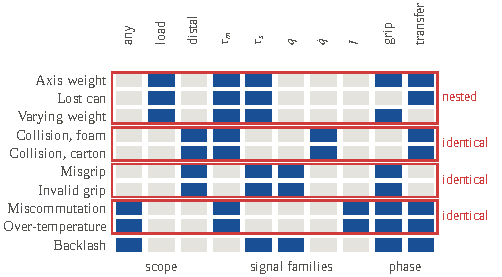
\includegraphics[width=\linewidth]{fig_signatures_column.pdf}
\caption{Knowledge-base columns of the nine modes in non-isolable groups and of
backlash, which has the gripping pair's families but not their scope. Families:
motor torque $\tau_m$, torque sensor $\tau_s$, joint position $q$, joint
velocity $\dot q$, current $I$; a phase hint `any' fills both phase cells.}
\label{fig:signatures}
\end{figure}

In 514 of the 755 anomalies (68.1\%) the top score is shared by two or three
modes, and every tie lies inside one group. 498 ties are in the load-torque
group: axis weight with lost can in 238 cycles, axis weight with varying weight
in 199, and all three in 61 cycles whose phase has no hint class. The other 16
are commutation-pair ties. The count is 514 for every phase weight from 0 to 3;
the weight changes only which members tie. These numbers describe this knowledge
base, not the robot: declaring the phase of axis weight as transfer instead of
any would leave 315 ties. What holds for any declarations is that no tie crosses
a group. The collision and gripping groups never reach rank one, because they
are declared on the wrist joints J4--J6, while the dominant joint, chosen by
absolute torque deviation, is J1, J2 or J3 in every cycle.

We route each cycle by the margin between its top score and the best score
outside its top group. Below $\tau = 0.15$, chosen on these cycles, it is
\emph{group-undetermined} (a reject option in the spirit of \citet{chow});
otherwise it is \emph{decisive} if its top group has one member and
\emph{human-resolvable} if it has several. The routes take 122, 134 and 499
cycles, with group accuracy 0.180, 0.187 and 0.421. Of the rejected cycles 82\%
are in the wrong group (80\% with $\tau$ chosen on training halves), against
66\% of all cycles.

%==============================================================================
\section{What the reported accuracy does not show}
\label{sec:baselines}
%==============================================================================

\subsection{The prevalence prior}

Against uniform chance, 0.071 over 14 modes, the deployed retrieval has a top-1
lift of 2.37$\times$, the figure we first reported. Uniform chance is the wrong
reference when categories differ in frequency: category~1 contributes 156 cycles
and category~8 contributes 10. The prevalence prior ranks the modes by their
frequency in the training half and gives this ranking for every cycle; it reads
no evidence.

\begin{table}[t]
\centering
\caption{Retrieval and references on the five test halves. Group: accuracy of
the predicted mode's group; for the prior, the most frequent group of the
training half. Balanced: mean per-category recall, with tied modes sharing the
credit; a constant scores $1/K$, with $K$ the 10 or 11 categories in a test
half. In parentheses: top-1 with tied modes sharing the credit. Two-stage:
Sec.~\ref{sec:repair}; flat classifier: Sec.~\ref{sec:neg}.}
\label{tab:baselines}
\small\setlength{\tabcolsep}{3.5pt}
\begin{tabular}{lcccc}
\toprule
& top-1 & top-5 & group & balanced \\
\midrule
uniform chance       & $0.071$ & $0.357$ & $0.150$ & $0.083$ \\
prevalence prior     & $0.187$ & $0.705$ & $0.401$ & $0.095$ \\
retrieval            & $0.169$ ($0.160$) & $0.651$ & $0.342$ & $0.105$ \\
\midrule
two-stage            & $0.309$ ($0.302$) & --- & $0.342$ & $0.208$ \\
flat classifier      & $0.525$ & --- & $0.574$ & $0.397$ \\
\bottomrule
\end{tabular}
\end{table}

Table~\ref{tab:baselines} compares the two. On top-3, top-5, MRR and group
accuracy the prior is ahead under every tie-break order of
Sec.~\ref{sec:tiebreak}; for top-3, MRR and group accuracy it is ahead on all
five splits. On top-1 the order decides. Under the declared order the retrieval
trails by 0.018 and is behind on four of five splits; under another order it is
ahead. Breaking ties by training-half frequency, which uses only the information
the prior uses, gives 0.200, level with the prior. Group accuracy does not favour
the retrieval either: always naming the most frequent group of the training
half, which is load torque on every split, scores 0.401 against 0.342.

Balanced recall, the mean of the per-category recalls, is the measure a
constant predictor cannot raise: a constant scores $1/K$, which averages 0.095.
The retrieval's balanced recall also depends on the tie-break, so we let tied
modes share the credit. The retrieval then reaches 0.105, above the constant on
every split but by only 0.003 to 0.016, and one order puts it below. It carries
per-cycle information, but little: its expected recall is zero on six of the
twelve categories. Comparisons between methods below use balanced recall in
this form.

\subsection{The tie-break interval}
\label{sec:tiebreak}

The scores do not determine which member of a tied set is reported; our
implementation reports the member declared first. Only five modes ever tie, always
within their group, so only $3!\cdot 2! = 12$ relative orders of the modes can
change the result. Fig.~\ref{fig:tiebreak} shows top-1 accuracy under all of
them. It ranges from 0.119 to 0.200, a width of 0.082. The declared order gives
0.169, and the mean over the orders, 0.160, equals the top-1 accuracy obtained
when tied modes share the credit \citep{mcsherry}. Two of the twelve orders reach
the prior's 0.187.

This spread is larger than the one due to the choice of split: over the orders
the five-split mean has standard deviation 0.027 and range 0.082, while the
declared-order value has standard deviation 0.015 and range 0.040 over the five
splits. More splits would not reduce the first, because one order applies to all
splits. Both ranges exceed the 0.018 by which the retrieval trails the prior. An
oracle that always picks the correct member of the tied set reaches 0.281. This
bounds rules that choose inside the tied set, but not rules that choose inside
the whole group, because the phase term has already removed the true mode from
46 tied sets.

The group of the top-ranked mode does not depend on the order: group accuracy is
0.342 under every tie-break rule, because no tie crosses a group. The group is
fixed, but it is not accurate. As a set it contains the true mode in 34.2\% of
cycles with 2.34 modes on average, while the same number of modes taken from the
top of the prevalence list contains it in 38.5\%. Only on balanced coverage is
the group ahead (0.243 against 0.222). The knowledge base fixes how coarse the
answer is, and the evidence does little to choose the group.

%==============================================================================
\section{Test selection over representation dimensions}
\label{sec:repair}
%==============================================================================

For each non-isolable group we ask which statistic of the existing signals, if
the representation carried it, would separate the members.

\emph{Dimensions.} The deployed representation keeps the peak magnitude
$\max|z|$ of each of the 26 record channels (\emph{mag}). The candidate
dimensions are further statistics of the same $z$: \emph{sign} (mean of $z$),
\emph{step} (last third of the cycle minus first third), \emph{payload} (carrying
minus empty actions), \emph{shape} (standard deviation of $z$) and
\emph{unread} (peak, signed and payload statistics of two channel families that
are recorded but not read by the attribution). Each has a cost class:
\emph{free} if computed from the record, \emph{pipeline} if it needs channels the
attribution does not read, \emph{hardware} if it needs a measurement the cell
does not have. None of our dimensions is of hardware class.

\emph{Search and certificate.} Every learned component is a standardised
$\ell_2$ logistic regression ($C = 1$). Starting from mag, a greedy search adds
the dimension with the largest gain in grouped inner cross-validation accuracy
on the training half ($k = \min(4,$ settings per class$)$ folds), as long as the
gain is at least $0.005$ times its cost factor (1 for free, 6 for pipeline). The
selected set is adopted on a split if its inner accuracy exceeds the
training-half majority rate by 0.05 and that of mag alone by 0.02; a group is
adopted if this holds on at least three of five splits. If a member has fewer
than two instantiations in the training half, no search can run; we then
evaluate the set of all free dimensions and do not adopt. The test half is only
reported: the certificate gives the dimensions, their cost class, the held-out
accuracy within the group and three controls (Table~\ref{tab:cert}). Varying the
cost factor, the minimum gain and both margins does not change which group is
adopted (repository).

\begin{table*}[t]
\centering
\caption{Repair certificates: accuracy within the group on held-out cycles of
its members. Grouped: leave-setting-out, the protocol we report. Ungrouped: the
same code under a random split over cycles, including its inner validation.
Deployed: the same classifier on the mag features alone. Majority: the
training-half majority rate. Permuted: the selected dimensions refitted on
training labels shuffled over cycles. Deployed, Majority and Permuted are
grouped. $^{\dag}$One carton instantiation in each training half, so no grouped
search can run; the value is for the set of all free dimensions.}
\label{tab:cert}
\small\setlength{\tabcolsep}{4pt}
\begin{tabular}{lcccccp{34mm}}
\toprule
Group & Ungrouped & Grouped & Deployed & Majority & Permuted & Verdict \\
\midrule
load torque (3 modes)      & $0.933$ & $0.840$ & $0.562$ & $0.504$ & $0.431$ &
  \textbf{adopted} on 5/5 splits, both protocols \\
distal collision (2 modes) & $0.830$ & $0.776^{\dag}$ & $0.709$ & $0.718$ & $0.608$ &
  \textbf{not adopted}: search cannot run; adopted ungrouped \\
gripping (2 modes)         & \multicolumn{5}{c}{one instantiation per member} &
  undetermined \\
commutation/temp (2 modes) & \multicolumn{5}{c}{no over-temperature instance in voraus-AD} &
  untestable \\
\bottomrule
\end{tabular}
\end{table*}

\textbf{Adopted.} Within the load-torque group the certificate reaches 0.840 on
held-out instantiations, against 0.562 for the deployed features, a majority
rate of 0.504 and 0.431 with permuted labels, and it is adopted on all five
splits. The dimension selected most often is sign (4 of 5 splits; step on 3,
unread and shape on 2 each), which mag does not contain. Because unread enters on
two splits, the certificate's worst-case cost class is pipeline, but the free set
\{sign, step\} reaches 0.869 against 0.872 for the best set with unread
channels, so no additional channel is needed. Most remaining errors are between
the two payload modes: on cycles of these two modes the resolver is right in
0.80 of cases, against 0.93 and 0.98 for the pairs with axis weight. These
figures are computed on cycles whose true mode is in the group, so they state
how well the repair works once a cycle reaches the group (Sec.~\ref{sec:route}).

\textbf{Not adopted.} Carton collision has three instantiations, so each
training half contains one and no grouped search can run. The set of all free
dimensions reaches 0.776 against a majority rate of 0.718. Each split trains on
one carton instantiation and tests on the other two, and three of the five splits
test on the same two, so the splits are not independent replications.
Sec.~\ref{sec:protocol} compares the protocols on this group with folds on which
the search can run.

\textbf{Undetermined.} Each gripping mode has one instantiation, so no grouped
split can test anything.

\textbf{Untestable.} voraus-AD contains no over-temperature fault, so this verdict
is assigned, not searched. The knowledge base names a separator for this pair,
current against torque for the same motion, which would be of pipeline cost.

End to end, the two-stage system (retrieval, then the resolver for cycles whose
top group is load torque) raises top-1 from $0.169 \pm 0.018$ to
$0.302 \pm 0.047$ with dimensions searched on each split. Fixing the dimensions
that most splits chose, \{sign, step\}, gives $0.309 \pm 0.031$, balanced recall
0.208 (from 0.105) and 0.869 within the group. That choice used all five splits;
made from the other four splits each time, it gives 0.301 and 0.846, so the
choice is worth less than 0.01. The gain over the retrieval is positive on every
split, from 0.089 to 0.151. It comes from the resolver, not from the routing:
sending every cycle to the load-torque resolver gives 0.349 and balanced recall
0.237, more than the two-stage system on all five splits.

%==============================================================================
\section{The validation protocol changes a deployment decision}
\label{sec:protocol}
%==============================================================================

Each \texttt{setting} value is one physical fault instantiation. A random split
over cycles therefore places cycles of the same instantiation in both halves,
and a model can learn to recognise the instantiation instead of the fault. The
methods react to the protocol as their use of labels predicts. The flat
classifier of Sec.~\ref{sec:neg} falls from 0.800 under a random split to 0.525
under leave-setting-out. The retrieval, which uses no labels, does not change
(0.161 and 0.162 over 20 splits of each kind).

For the load-torque group the certificate is adopted under both protocols
(Table~\ref{tab:cert}). For the collision group the protocols disagree. Under a
random split the inner validation, whose folds share instantiations, reaches
0.85 to 0.96, and the repair is adopted on all five splits, although on held-out
cycles it beats the majority class of the same split by only 3 of 47 cycles
(0.830 against 0.766). Under the 50/50 leave-setting-out split no grouped search
can run (Sec.~\ref{sec:repair}), so we compare the protocols with nine folds and
the same search and rule. With folds stratified over cycles, the repair is
adopted on 9 of 9 folds. With one setting held out per fold, it is adopted on 4
of 9 folds, and its pooled held-out accuracy is 0.67 to 0.75 over ten inner
seeds, below the majority rate of 0.766 for every seed.

A permuted-label control that shuffles labels over cycles does not detect the
difference, because the shuffled labels are still learned from cycles of the same
instantiations. Permuting labels over whole settings does: under the random
split, between 5 and 10 of the 84 possible labellings reach the observed
collision accuracy on each split ($p = 0.06$ to $0.12$), while none of 300
labellings reaches the load-torque accuracy ($p < 0.004$). Any learned
comparison on this benchmark should therefore group by setting in the inner
validation as well as in the outer split.

%==============================================================================
\section{Controls, and what would settle the open verdicts}
\label{sec:neg}
%==============================================================================

\subsection{The flat classifier}

A flat 12-way logistic regression over all dimensions reaches 0.525 top-1,
0.397 balanced recall and 0.574 group accuracy under the same protocol, against
0.309, 0.208 and 0.342 for our system. We tested whether the knowledge base at
least saves labels. Over 20 paired leave-setting-out splits, the classifier is
trained on $k$ labelled cycles and the two-stage system on $k$ labelled cycles
per group; only the load-torque group receives cycles, so only its labels are
used. Both are scored on the twelve-way task. At $k = 3$ the two-stage system, which is then close to the
knowledge base alone, has the higher balanced recall on 17 of 20 splits. From
$k = 8$ the classifier has the higher top-1 (0.225 against 0.208, 15 of 20
splits), from $k = 12$ also the higher balanced recall (17 of 20), and at
$k = 320$ it reaches 0.550 against 0.304. If the two-stage system receives the
same random labels as the classifier, it is behind at $k = 8$ on all 20 splits.
Where more than a few labels can be collected, the flat classifier is the better
choice; the advantage of the knowledge base is limited to the case with almost
no labels.

\subsection{Where the ranking's output goes}
\label{sec:route}

The load-torque group is the true answer for 41.1\% of cycles but is ranked
first for 66.0\%. Of the cycles it receives, 58\% are not load-torque faults.
The resolver is right on 0.88 of the true members it receives, so the route as a
whole is right on 0.37, against 0.16 for the retrieval alone on the same cycles.
The collision and gripping groups are the true answer for 12.5\% and 3.0\% of
cycles and are ranked first for none (Sec.~\ref{sec:twins}), so for them there
is no route to measure; their certificates state whether a repair would work if
the group were reached. The flat classifier recognises foam collision in 0.506
of cases, a category on which the retrieval and the prior both score zero, so
the features contain evidence that the attribution and the retrieval do not use.

\subsection{What would settle the open verdicts}

Gripping has one instantiation per mode, so no grouped protocol can evaluate it.
For collision the limit is our split: a 50/50 grouped split leaves
$\lfloor N/2 \rfloor$ instantiations per mode for training, the grouped inner
search needs two, and carton has $N = 3$. With one setting held out at a time
the search runs and is still not adopted (Sec.~\ref{sec:protocol}). Sweeps over
$N$ on injected faults and on a simulated cell are in the repository; in both
the deployed features already separate the pair, so they do not show how many
instantiations a real non-isolable pair needs.

%==============================================================================
\section{Conclusion}
%==============================================================================

On voraus-AD the ranked list of an FMEA-based diagnosis layer is limited by its
knowledge base before any data are scored: 68.1\% of anomalies tie at rank one,
almost all in the load-torque group. A single top-1 figure then depends on the
tie-break order more than on the method, and a prevalence prior is better on
every measure that does not depend on the order.

We therefore report the non-isolable group and search for a statistic that
separates it, with held-out evidence, controls and a cost class. One of the
three groups with benchmark instances is separated on unseen instantiations, by
the sign of the deviation at no extra cost. This search must be validated by
instantiation: a random split adopts a collision repair that leave-setting-out
validation does not, and a permuted-label control over cycles does not notice.

Whether a candidate list can decide can be checked before any data are seen,
but a list that decides is not therefore more accurate. Adding the knowledge
base's own declarations of torque direction and step to the score removes 513
of the 514 ties but lowers balanced recall on four of five splits (0.105 to
0.100) and top-1 on all five. A change of representation should be adopted on
evidence from unseen instantiations, not because it makes the list decidable.

% Final manuscripts are limited to SIX pages under the post-2022 IFAC policy,
% with no over-length allowance.  This file is built to that limit, not to the
% eight pages the review stage permits.
% The DOI below should be the Zenodo CONCEPT doi (resolves to the latest
% version), not a version-specific one, so the citation does not go stale when
% the deposit is updated.  Check on the Zenodo record page under "Cite all
% versions" before submitting.

\emph{Code and data.} Evidence records, certificates, all analyses and the
producing scripts are archived at
\mbox{\url{https://doi.org/10.5281/zenodo.22089173}}.

%==============================================================================
\begin{thebibliography}{99}
\small
\setlength{\itemsep}{0pt}
\setlength{\parsep}{0pt}
\linespread{0.96}\selectfont

% ---------------------------------------------------------------------------
% 18 entries.  Every one is cited in the text -- no padding.  All bibliographic
% details (volume, issue, pages, DOI) were checked against the publisher record
% or the authors' own publication lists.  Do not add an entry you have not
% opened yourself.
% CHECK: hendriks, jung18 and mcsherry were added in the October revision; their
% details were confirmed from secondary listings only.  Open each before
% submission.
% ---------------------------------------------------------------------------

\bibitem[Blanke et al.(2016)]{blanke}
Blanke, M., Kinnaert, M., Lunze, J., and Staroswiecki, M. (2016).
\emph{Diagnosis and Fault-Tolerant Control}, 3rd ed. Springer, Berlin.

\bibitem[Brockmann et al.(2024)]{voraus}
Brockmann, J.T., Rudolph, M., Rosenhahn, B., and Wandt, B. (2024).
The voraus-AD dataset for anomaly detection in robot applications.
\emph{IEEE Transactions on Robotics}, 40, 438--451.

\bibitem[Chow(1970)]{chow}
Chow, C.K. (1970).
On optimum recognition error and reject tradeoff.
\emph{IEEE Transactions on Information Theory}, 16(1), 41--46.

\bibitem[Cordier et al.(2004)]{cordier}
Cordier, M.-O., Dague, P., L\'{e}vy, F., Montmain, J., Staroswiecki, M., and
Trav\'{e}-Massuy\`{e}s, L. (2004).
Conflicts versus analytical redundancy relations: a comparative analysis of the
model based diagnosis approach from the artificial intelligence and automatic
control perspectives.
\emph{IEEE Transactions on Systems, Man, and Cybernetics --- Part B}, 34(5),
2163--2177.

\bibitem[de Kleer and Williams(1987)]{dekleer}
de Kleer, J. and Williams, B.C. (1987).
Diagnosing multiple faults.
\emph{Artificial Intelligence}, 32(1), 97--130.

\bibitem[D\"{u}steg\"{o}r et al.(2006)]{damadics}
D\"{u}steg\"{o}r, D., Frisk, E., Cocquempot, V., Krysander, M., and
Staroswiecki, M. (2006).
Structural analysis of fault isolability in the DAMADICS benchmark.
\emph{Control Engineering Practice}, 14(6), 597--608.

\bibitem[Frisk et al.(2009)]{frisk}
Frisk, E., Krysander, M., and \r{A}slund, J. (2009).
Sensor placement for fault isolation in linear differential-algebraic systems.
\emph{Automatica}, 45(2), 364--371.

\bibitem[Hendriks et al.(2022)]{hendriks}
Hendriks, J., Dumond, P., and Knox, D. (2022).
Towards better benchmarking using the CWRU bearing fault dataset.
\emph{Mechanical Systems and Signal Processing}, 169, 108732.

\bibitem[Jung et al.(2015)]{jung}
Jung, D., Frisk, E., and Krysander, M. (2015).
Quantitative isolability analysis of different fault modes.
\emph{IFAC-PapersOnLine}, 48(21), 1275--1282.

\bibitem[Jung et al.(2018)]{jung18}
Jung, D., Ng, K.Y., Frisk, E., and Krysander, M. (2018).
Combining model-based diagnosis and data-driven anomaly classifiers for fault
isolation. \emph{Control Engineering Practice}, 80, 146--156.

\bibitem[Kapoor and Narayanan(2023)]{kapoor}
Kapoor, S. and Narayanan, A. (2023).
Leakage and the reproducibility crisis in machine-learning-based science.
\emph{Patterns}, 4(9), 100804.

\bibitem[Krysander and Frisk(2008)]{krysander}
Krysander, M. and Frisk, E. (2008).
Sensor placement for fault diagnosis.
\emph{IEEE Transactions on Systems, Man, and Cybernetics --- Part A}, 38(6),
1398--1410.

\bibitem[Krysander et al.(2008)]{krysander_mso}
Krysander, M., \r{A}slund, J., and Nyberg, M. (2008).
An efficient algorithm for finding minimal overconstrained subsystems for
model-based diagnosis.
\emph{IEEE Transactions on Systems, Man, and Cybernetics --- Part A}, 38(1),
197--206.

\bibitem[Liao et al.(2025)]{aei_kg}
Liao, X., Chen, C., Wang, Z., Liu, Y., Wang, T., and Cheng, L. (2025).
Large language model assisted fine-grained knowledge graph construction for
robotic fault diagnosis.
\emph{Advanced Engineering Informatics}, 65, 103134.

\bibitem[McSherry and Najork(2008)]{mcsherry}
McSherry, F. and Najork, M. (2008).
Computing information retrieval performance measures efficiently in the
presence of tied scores. In \emph{Advances in Information Retrieval (ECIR
2008)}, LNCS 4956, 414--421. Springer.

\bibitem[Reiter(1987)]{reiter}
Reiter, R. (1987).
A theory of diagnosis from first principles.
\emph{Artificial Intelligence}, 32(1), 57--95.

\bibitem[Trav\'{e}-Massuy\`{e}s(2014)]{tm_survey}
Trav\'{e}-Massuy\`{e}s, L. (2014).
Bridging control and artificial intelligence theories for diagnosis: a survey.
\emph{Engineering Applications of Artificial Intelligence}, 27, 1--16.

\bibitem[Trav\'{e}-Massuy\`{e}s and Wotawa(2024)]{tm_wotawa}
Trav\'{e}-Massuy\`{e}s, L. and Wotawa, F. (2024).
Bridging hardware and software diagnosis: leveraging fault signature matrix and
spectrum-based fault localization similarities.
In \emph{35th International Conference on Principles of Diagnosis and Resilient
Systems (DX 2024)}, OASIcs vol. 125, 5:1--5:15.

\end{thebibliography}

\end{document}
